\chapter{Diseño e implementación}
\label{cap:DisenioImplementacion}

En este capítulo se presenta la arquitectura de hardware y software del dispositivo de captura, como así también del generador de señal MVB desarrollado para probar el dispositivo de captura sin necesidad de conectarlo en una formación ferroviaria.

\section{Arquitectura de hardware}
\label{sec:hardware}

Como se muestra en la figura~\ref{fig:conexion}, el dispositivo de captura tiene dos conectores DE-9 compatibles con el medio EMD. De esta manera se lo puede conectar a un segmento MVB entre dos dispositivos cualesquiera.

\begin{figure}[htbp]
	\centering
    {
        \fontfamily{phv}
        \fontsize{8pt}{8pt}\selectfont
        \input{./Figures/conexion.pdf_tex}
    }
	\caption{Conexión del dispositivo de captura en un segmento EMD.}
    \label{fig:conexion}
\end{figure}

En la figura~\ref{fig:bloques} se muestra un diagrama de la arquitectura del dispositivo de captura.
Se dejan en corto circuito las líneas de transmisión (ver figura~\ref{fig:pines}), de forma tal de que el dispositivo opere en forma pasiva, y sea transparente para el resto de los dispositivos del segmento.
El dispositivo MAX485 \cite{max485} se utiliza para convertir la señal de entrada (par diferencial $-$5~V - +5~V) a una señal compatible para el analizador lógico VKTECH (0~V - +5~V). El analizador lógico se conecta a una Raspberry Pi mediante un puerto USB 2.0. La Raspberry Pi decodifica las tramas por software y almacena los datos capturados en una tarjeta de memoria. Mediante su interfaz Wi-Fi se puede conectar una PC (utilizando el protocolo SSH) para descargar las capturas, y también para visualizar el tráfico del bus MVB en tiempo real.

\begin{figure}[htbp]
	\centering
    {
        \fontfamily{phv}
        \fontsize{8pt}{8pt}\selectfont
        \input{./Figures/bloques.pdf_tex}
    }
	\caption{Arquitectura de hardware del dispositivo de captura.}
    \label{fig:bloques}
\end{figure}

En la figura~\ref{fig:esquematico} se muestra un diagrama esquemático con el detalle de las conexiones entre los diferentes componentes. En el diagrama se utiliza la etiqueta ``USB'' para representar la conexión a la Raspberry Pi, que no se muestra por simplicidad. Asímismo, la conexión ``VCC'' del MAX485 se conecta al pin número 2 del conectpr GPIO de la Raspberry Pi \cite{gpio}.

\begin{figure}[htbp]
	\centering
	\includegraphics[width=1\textwidth]{./Figures/esquematico.png}
	\caption{Diagrama esquemático del dispositivo de captura.}
    \label{fig:esquematico}
\end{figure}

En la figura~\ref{fig:fotodispositivo} se muestra una foto del dispositivo de captura en construcción.

\begin{figure}[htbp]
	\centering
	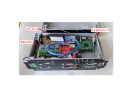
\includegraphics[width=1\textwidth]{./Figures/foto-dispositivo.pdf}
	\caption{Foto del dispositivo de captura en construcción.}
    \label{fig:fotodispositivo}
\end{figure}

\section{Arquitectura de software}
\label{sec:software}

\section{Dispositivo generador de señal}
\label{sec:generador}
